\section{DPCM}


\begin{frame}%[allowframebreaks]
  \frametitle{DPCM}
  O DPCM (\textit{Differential pulse-code modulation}) foi criado 1950 por Cassius Chapin Cutler.
  O codificador utiliza um preditor linear para o sinal a ser codificado. O erro de predição é quantizado e transmitido/armazenado.
  Para a decodificação utiliza-se o mesmo preditor e soma-se o erro de predição recebido na entrada do decodificador.
\end{frame}

\begin{frame}%[allowframebreaks]
  \frametitle{DPCM - Codificador e Decodificador}
  \begin{columns}[c]
  \column{.5\textwidth}
  \begin{figure}[h!]
  \centering
  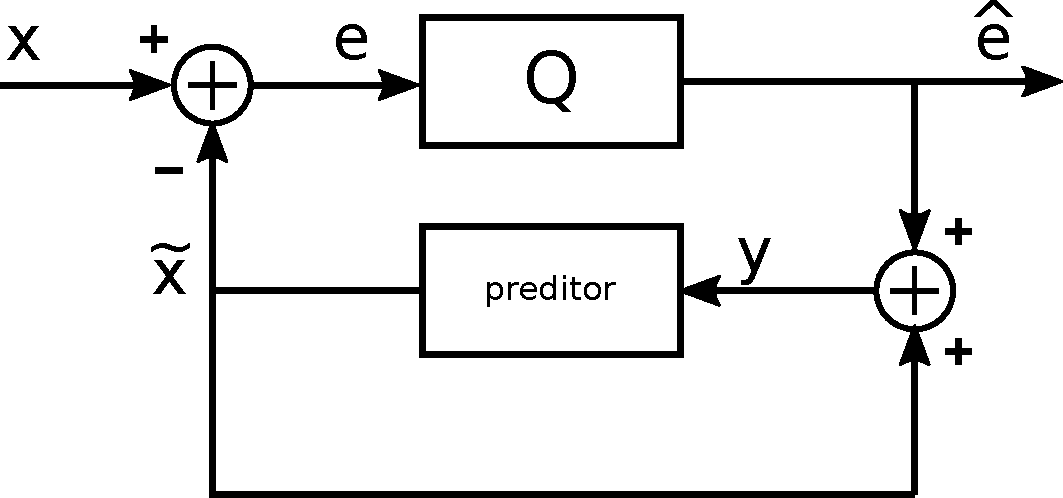
\includegraphics[width=0.9\textwidth]{images/dpcm_codificador.pdf}
  \caption{Codificador DPCM.}
  \label{fig:dpcm_enc}
  \end{figure}
  \column{.5\textwidth}
  \begin{figure}[h!]
  \centering
  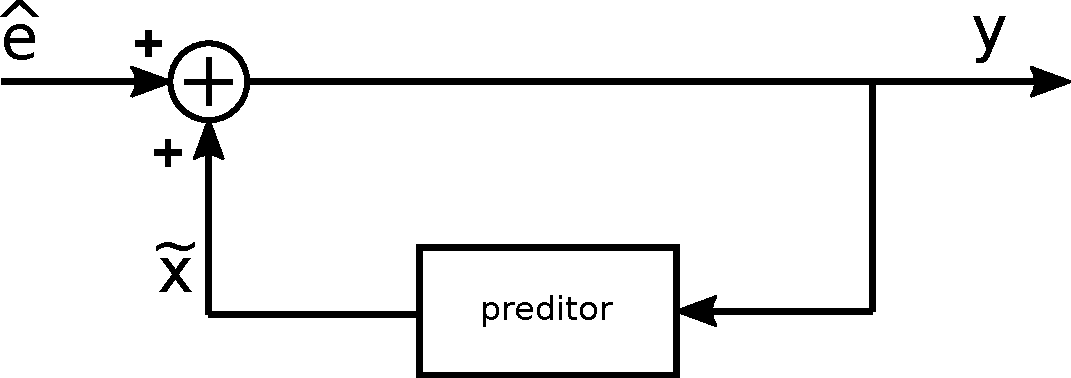
\includegraphics[width=0.9\textwidth]{images/dpcm_decodificador.pdf}
  \caption{Decodificador DPCM.}
  \label{fig:dpcm_denc}
  \end{figure}
  \end{columns}

\end{frame}


\begin{frame}%[allowframebreaks]
  \frametitle{DPCM - exemplo}

  \centering
  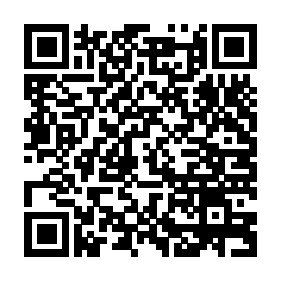
\includegraphics[width=0.3\textwidth]{images/qrcode-jupyter-dpcm.pdf}
  \url{https://nbviewer.jupyter.org/github/leolca/notebooks/blob/master/aev/dpcm_example_image.ipynb}

\end{frame}

\begin{frame}
  \frametitle{Leitura}
  Sugestão de leitura:
  \begin{itemize}
  \item \bibentry{salomon2010}
  \item \bibentry{yehia1993}
  \end{itemize}
\end{frame}
